\documentclass[12pt,oneside]{article}

\usepackage[english]{babel} 
\usepackage[T1]{fontenc}
\usepackage{a4}
\usepackage{indentfirst}
\usepackage{fancyhdr}
\usepackage{graphicx}
\usepackage{hyperref}
\hypersetup{colorlinks,urlcolor=blue}
\usepackage{subfigure}
\usepackage[hang,small,bf]{caption}
\setlength{\captionmargin}{20pt}
\captionsetup{justification=raggedright,singlelinecheck=false}
\usepackage{wrapfig}
\usepackage{url}
\urlstyle{rm}
\usepackage[svgnames]{xcolor}
\usepackage{pgfplots}
\pgfplotsset{width=0.40\textwidth, compat=1.6}
\usepgfplotslibrary{groupplots}
\hyphenation{vo-lu-me}
\usepackage[margin=1.5cm]{geometry}
\setlength\parindent{10cm}
\usepackage{tikz}
\usepackage[bottom]{footmisc}
\usepackage{xurl}
\usepackage{seqsplit}
\usepackage{lmodern}

\begin{document}

\noindent
\pagestyle{empty}

%%%%%%%%% Sustain Results %%%%%%%%%%%%%%

\section*{Subject subtyping and staging \footnote{{Young et al. Uncovering the heterogeneity and temporal complexity of neurodegenerative diseases with Subtype and Stage Inference. Nat Commun 9, 4273 (2018).}}}
\noindent

\begin{table}[h!]
\begin{tabular}{p{0.55\textwidth}p{0.35\textwidth}} 
\vspace{-3.5cm}
\begin{tabular}{l p{0.3\textwidth}}
\textbf{Scan Name:} & \textit{\expandafter\seqsplit\expandafter{\detokenize{@@IDDDD@@}}}\\
\textbf{Sex:} & \textit{@@SSEXX@@} \\
\textbf{Age:} & $@@AGGGE@@$ \\
\textbf{Atrophy pattern: } & \textit{@@SUBTP@@} \textit{(}$@@SUBPB@@\%$ \textit{probability)}\\
\textbf{Model stage: } & $@@STAGE@@$ 
\end{tabular}
&
\includegraphics[width=6cm]{Histo.png}
\end{tabular}
\end{table}

%%%%%%%comment%%%%

@@COMMT@@

%%%%%%%brainpainter%%%%%

\begin{figure*}[b!]
\centering
{\includegraphics[height=0.19\textwidth]{cort_inn.png}}
{\includegraphics[height=0.19\textwidth]{cort_out.png}}
{\includegraphics[height=0.19\textwidth]{sub_cort.png}}
{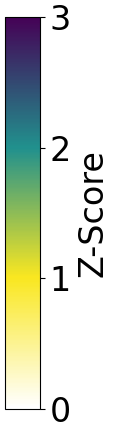
\includegraphics[height=0.19\textwidth]{legend.png}}
\vspace{-0.3cm}
\caption*{\textbf{Fig.2:} Atrophy z-scores for the relevant brain regions. From left to right: cortical inner view, cortical outer view, subcortical view. Images were generated using \href{https://arxiv.org/abs/1905.08627}{Brainpainter}}
\end{figure*}

\end{document}
